\documentclass[10pt, twocolumn, letterpaper]{article}

\usepackage[utf8]{inputenc}
\usepackage{geometry}
\geometry{margin=0.75in}
\usepackage{times}
\usepackage{graphicx}
\usepackage{amsmath}
\usepackage{amssymb}
\usepackage{booktabs}
\usepackage{algorithm}
\usepackage{algpseudocode}
\usepackage{hyperref}
\usepackage{xcolor}
\usepackage{float}
\usepackage{tikz}
\usetikzlibrary{shapes, arrows.meta, positioning, fit, calc}

% Title and Author
\title{\textbf{LifeLink: Resilient Mesh Communication in Spectrally Contested Environments \\ via Semantic Compression and Economic Asymmetry}}

\author{
  \textbf{The LifeLink Team} \\
  Stanford TreeHacks 2026 \\
  \texttt{raghavt3@illinois.edu} \\
  \texttt{tkoduru@umich.edu} \\
  \texttt{rohan@WPI.edu} \\
  \texttt{vijay@stanford.edu} \\
}

\date{}

\begin{document}

\maketitle

\begin{abstract}
In modern conflict zones and disaster scenarios, civilians face a dual threat: the physical destruction of infrastructure and the active suppression of wireless communications. Adversaries increasingly deploy jamming to deny Wi-Fi/Cellular connectivity and GPS spoofing to disrupt navigation. We present \textbf{LifeLink}, a decentralized communication architecture designed for these Anti-Access/Area Denial (A2/AD) environments. By utilizing LoRa (915 MHz) hardware, we bypass high-frequency jamming, but incur severe bandwidth constraints. To solve this, we introduce \textit{Semantic Compression}—an edge-AI triage system that reduces natural language to 8-byte payloads. We further demonstrate that LifeLink creates an "Asymmetric Cost Exchange," where the financial and tactical cost to jam the network effectively exceeds the cost of deployment by orders of magnitude.
\end{abstract}

\section{Introduction: The Spectral Denial Problem}
Standard emergency communication systems rely on two assumptions: reliable high-bandwidth backhaul (Cellular/Wi-Fi) and reliable positioning (GPS). In contested environments, both assumptions fail.

\subsection{The Jamming Threat Model}
\begin{enumerate}
    \item \textbf{High-Frequency Denial:} 2.4GHz and 5GHz bands (Wi-Fi) are easily attenuated by walls and effectively jammed by low-cost wide-band interrupters.
    \item \textbf{GNSS Denial:} GPS signals are weak (-125 dBm) and susceptible to spoofing or jamming, rendering standard location-sharing apps useless.
\end{enumerate}

To address this, LifeLink shifts the physical layer to LoRa (Long Range) at 915 MHz. This lower frequency offers superior penetration through urban obstacles and is significantly harder to jam without high-power military-grade equipment. However, this shift reduces available bandwidth from Megabits/sec to roughly 300 bits/sec. This physical constraint necessitates our primary contribution: \textit{Semantic Compression}.

\section{The Economics of Suppression}
A key design goal of LifeLink is to leverage the asymmetry of cost between the \textit{suppressor} (the jammer) and the \textit{communicator} (the node). We utilize Commodity-Off-The-Shelf (COTS) hardware ($\approx$\$5/node at scale) to force the adversary into a Game Theoretic loss condition.

We define the suppression game outcomes as follows:
\begin{enumerate}
    \item \textbf{Scenario A (Zero Deployment):} If the adversary deploys no jammers, LifeLink operates as a standard high-availability mesh.
    \item \textbf{Scenario B (Partial Denial):} If the adversary deploys limited jamming, the mesh topology is able to dynamically route around interference holes. The low cost of nodes allows civilians to "swarm" the environment, ensuring that a signal path exists statistically.
    \item \textbf{Scenario C (Total Saturation):} To fully suppress a city-scale LoRa mesh, the adversary must blanket the noise floor across the entire 900MHz spectrum. This incurs an astronomical power cost and, critically, denies the adversary use of the spectrum for their own communications.
\end{enumerate}

\section{Hardware Architecture}
The physical node is designed for zero-maintenance operation. It functions entirely off-grid, harvesting solar energy to maintain a continuous listening state.

\subsection{Electrical Schematic}

The main purpose of our electrical system, which can be seen in the node wiring diagram below, is to mediate between the bursts of power provided by the solar panel through the use of a standard lipo cell.

% FIXED: Added resizebox to scale image to column width
\begin{figure}[H] 
\centering
\resizebox{\columnwidth}{!}{%
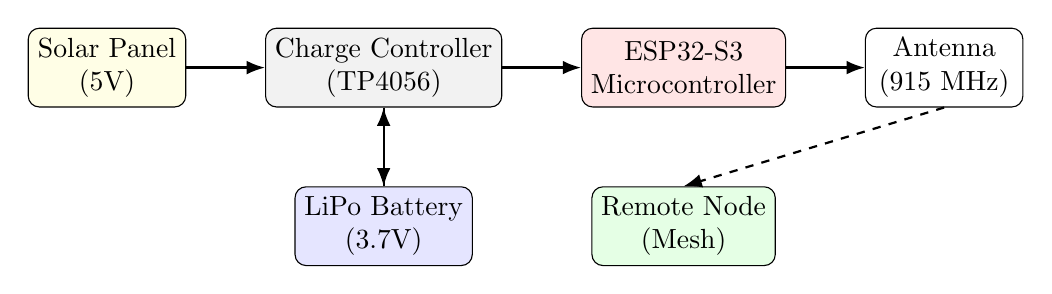
\begin{tikzpicture}[
    node distance=1cm and 1cm,
    block/.style={rectangle, draw, rounded corners, minimum width=2cm, minimum height=1cm, align=center},
    line/.style={-Latex, thick},
    wireless/.style={-Latex, dashed, thick}
]

% Nodes
\node[block, fill=yellow!10] (solar) {Solar Panel\\(5V)};
\node[block, right=of solar, fill=gray!10] (controller) {Charge Controller\\(TP4056)};
\node[block, below=of controller, fill=blue!10] (battery) {LiPo Battery\\(3.7V)};
\node[block, right=of controller, fill=red!10] (esp) {ESP32-S3\\Microcontroller};
\node[block, right=of esp] (antenna) {Antenna\\(915 MHz)};
\node[block, below=of esp, fill=green!10] (other) {Remote Node\\(Mesh)};

% Connections
\draw[line] (solar) -- (controller);
\draw[line] (controller.south) -- (battery.north);
\draw[line] (battery.north) -- (controller.south);
\draw[line] (controller) -- (esp);
\draw[line] (esp) -- (antenna);
\draw[wireless] (antenna.south) -- (other.north);

\end{tikzpicture}%
}
\caption{\textbf{Node Wiring Diagram.} The Charge Controller isolates the LiPo from over-discharge while regulating Solar input. The ESP32 handles the Protocol Stack and drives the RF interface.}
\label{fig:hardware}
\end{figure}

\section{Methodology: Semantic Compression}
Since we cannot transmit full text over LoRa during high congestion, we implement an AI-driven compression layer.

\subsection{Feature Engineering for Embedded Systems}
We utilize a lightweight vectorizer suitable for the ESP32's constraints. An input string $S$ is mapped to a feature vector $V \in \mathbb{R}^{82}$ composed of three subspaces:
\begin{equation}
    V = [v_{struct} \parallel v_{intent} \parallel v_{ngram}]
\end{equation}

While $v_{struct}$ captures morphology (e.g., capitalization ratio, punctuation), the critical innovation is $v_{ngram}$. To avoid storing a large vocabulary on the microcontroller, we employ the \textbf{FNV-1a} hash function. Character 4-grams are hashed into 64 fixed bins:
\begin{equation}
    v_{ngram}[i] = \sum_{g \in \text{grams}} \mathbb{I}(\text{FNV1a}(g) \pmod{64} = i)
\end{equation}
This allows the model to learn semantic clusters (e.g., "help", "hlp", "plz") robustly without a dictionary.

\subsection{Hierarchical Triage}
Inference uses a cascaded Decision Tree ensemble. A binary "Gate" classifier first determines if the message is \textit{Vital}. If true, secondary classifiers predict \textit{Intent} (e.g., MEDIC, EVAC) and \textit{Urgency} ($U \in [0,3]$).

This reduces a 100-byte SMS to a rigid schema:
\begin{equation}
    \text{Payload} = \texttt{INTENT} \mid U_3 \mid F_{flags} \mid N_{count} \mid L_{token}
\end{equation}
This payload is approximately 8 bytes, reducing Airtime Utilization by $>90\%$ for critical traffic.

\section{Protocol: Hybrid Resilient Routing}
LifeLink implements a custom OSI Layer 3 protocol that does not rely on static routing tables.

\subsection{Epidemic Gossip}
Topology discovery is achieved via "piggybacking." Every heartbeat packet carries a compressed list of the sender's known neighbors. When Node $A$ receives a heartbeat from Node $B$, it updates its internal cost matrix:
\begin{equation}
    Cost(A \to D) = \min(Cost_{curr}, Cost(B \to D) + 1)
\end{equation}
This propagates connectivity data exponentially ("Epidemic" spread) without flooding the network with control packets.

\subsection{Geographic-Gradient Forwarding}
Routing decisions for a packet at Node $N$ destined for $D$ follow a prioritized heuristic:
\begin{enumerate}
    \item \textbf{Direct Delivery:} If $D$ is a neighbor, transmit directly.
    \item \textbf{Geographic Greedy:} If $N$ has high position confidence ($C > 0.3$), forward to the neighbor $n$ that minimizes the Haversine distance to $D$:
    \begin{equation}
        n^* = \operatorname*{argmin}_{n \in Neighbors} \text{Haversine}(Pos_n, Pos_D)
    \end{equation}
    \item \textbf{Gradient Fallback:} If Geographic forwarding encounters a local minima (no neighbor is closer), the protocol falls back to the "Hops Away" gradient learned via gossip.
\end{enumerate}

\section{Simulation Engine: Physical Fidelity and Robustness}
We implement a deterministic, tick-based network simulator (1 tick $\approx$ 100ms at 1$\times$ speed) that separates \textit{protocol logic} from \textit{RF environment physics}. This allows controlled stress-testing under contention, jamming, and topology churn.

\subsection{Discrete-Time Execution Model}
At each tick, the engine executes the following ordered phases:
\begin{enumerate}
    \item \textbf{Environment Update:} clear previous in-air signals and decay interference memory.
    \item \textbf{FTM Ranging Phase:} non-anchor nodes range all neighbors within FTM radius.
    \item \textbf{Node Loop:} each node performs neighbor expiry, trilateration update, gossip/heartbeat scheduling, and trust-aware routing state updates.
    \item \textbf{Transmit Phase:} each node can emit at most one packet per tick (half-duplex TX/RX simplification).
    \item \textbf{Receive Phase:} each listening node resolves all on-channel candidates using SNR and capture/collision logic.
\end{enumerate}
This strict ordering makes experiments reproducible and prevents event-order ambiguity common in asynchronous simulators.

\subsection{Propagation, Noise, and Jamming Model}
For a transmitter at distance $d$ (meters), received power is modeled with log-distance path loss:
\begin{equation}
    RSSI(d) = P_{tx} - 40 - 20\log_{10}(\max(d,1))\ \text{dBm}
\end{equation}
where $P_{tx}$ defaults to 20 dBm. A receiver considers only transmitters within fixed radio radius $R_{LoRa}$.

Total effective noise is:
\begin{equation}
    N_{tot} = N_0 + J(d,c) + I_c\cdot 20
\end{equation}
where $N_0$ is baseline noise floor, $J(d,c)$ is channel-specific jammer contribution, and $I_c \in [0,1]$ is per-channel interference memory. A single-link decode requires:
\begin{equation}
    SNR = RSSI - N_{tot} > 0
\end{equation}
otherwise the packet is marked jammed.

\subsection{Collision and Capture Effect}
For multiple simultaneous candidates on the same channel, we sort by RSSI and apply capture-effect decoding. Let $P_1$ and $P_2$ be strongest and second-strongest packets:
\begin{equation}
    \Delta = RSSI_1 - RSSI_2
\end{equation}
If $\Delta \geq 6$ dB, $P_1$ is decoded (status \textit{captured}) and others collide; else all collide. This mirrors practical near-far behavior in low-rate links and gives realistic partial-survival under congestion.

\subsection{Localization and Topology Estimation}
Positioning uses hybrid anchor + FTM ranging:
\begin{enumerate}
    \item Pairwise FTM distance measurements are simulated with Gaussian measurement noise ($\sigma\approx 0.8$m).
    \item Nodes collect at least three confident anchor/peer references.
    \item Position is solved by iterative damped least-squares trilateration (Gauss-Newton style).
    \item Confidence increases with anchor count and decays through multi-hop gossip.
\end{enumerate}
This explicitly separates \textit{true physics coordinates} (simulator ground truth) from \textit{estimated coordinates} (what the node believes), enabling localization-error-aware routing behavior.

\subsection{Routing, Gossip, and Trust Constraints}
Routing is trust-aware geographic-gradient forwarding:
\begin{enumerate}
    \item direct neighbor delivery if destination is one hop away,
    \item geographic greedy forwarding if destination position confidence is sufficient,
    \item gradient fallback via learned \textit{via-node} from gossip,
    \item fail if no admissible next hop exists.
\end{enumerate}
Gossip heartbeats carry compressed neighbor entries, allowing epidemic-style membership propagation without dedicated control floods. TTL bounds and dedup buffers constrain loop persistence.

\subsection{Scalability Characteristics}
The simulator is designed to model city-scale behavior trends, while remaining computationally tractable for browser-based experimentation:
\begin{itemize}
    \item \textbf{FTM phase:} naive all-pairs proximity check is $\mathcal{O}(N^2)$ per tick.
    \item \textbf{Receive phase:} for each node, decoding cost scales with in-range on-channel contenders; worst-case dense contention approaches $\mathcal{O}(N^2)$.
    \item \textbf{Traffic shaping:} one TX dequeue per node per tick prevents unbounded queue explosion and stabilizes runtime under burst injection.
    \item \textbf{Memory bounds:} bounded dedup buffers, capped gossip entries, and finite event/transmission logs prevent unbounded state growth.
\end{itemize}
Thus, the framework is primarily a \textit{mesoscopic} simulator: suitable for robust comparative studies (protocol variants, jamming strategies, trust policies), while abstracting away waveform-level PHY details.

\subsection{Validation and Robustness Test Matrix}
We validate correctness and resilience using scenario-driven tests with observable metrics:
\begin{itemize}
    \item \textbf{Delivery Path Metrics:} total sent, delivered, dropped, collisions, and average hop count.
    \item \textbf{Topology Convergence:} membership coverage (fraction of known peers) under varying beacon jitter and churn.
    \item \textbf{Adversarial Stress:} multi-channel jammers with varying radius/power to evaluate degradation mode (jammed vs captured vs collision).
    \item \textbf{State Robustness:} trust graph persistence across simulator resets triggered by node-set changes, ensuring configured trust edges are not lost during topology updates.
\end{itemize}
The trust-persistence fix is critical for experimental validity: without it, adding nodes mutates security topology unintentionally, confounding comparisons across runs.

\subsection{Model Limitations (Explicit)}
To avoid overstating claims, we explicitly note current abstractions:
\begin{enumerate}
    \item fixed-range cutoff rather than probabilistic reception curves,
    \item no fading, shadowing maps, Doppler, or coding-rate/SF adaptation,
    \item simplified half-duplex scheduling and per-tick synchronization,
    \item simplified trust/crypto semantics for protocol experimentation.
\end{enumerate}
These choices intentionally prioritize reproducibility, parameter sweeps, and systems-level insight over waveform-level emulation.

\section{Conclusion}
LifeLink validates that civilian communication infrastructure can be hardened against state-level disruption. By combining the physics of LoRa propagation, the economics of cheap hardware, and the efficiency of semantic AI, we render the strategy of spectral jamming fiscally and tactically obsolete.

\end{document}
